% Chapter 3

\chapter{Experimental Set Up} % Main chapter title

\label{Chapter3} % For referencing the chapter elsewhere, use \ref{Chapter3} 
In the interest of reproducibility we include in this section some of the considerations specific to our data set. Additionally we cover the data pre-processing steps taken prior to our experiments and describe our process for model tuning. Finally, we outline the procedure taken for the classification and clustering experiments. 

%----------------------------------------------------------------------------------------
\section{Considerations}

% THE DATASET
The data we used for our experiments comes from the August 2015 EPO Worldwide Patent Statistical Database (\keyword{PATSTAT}). According to the EPO, this data set contains over 90 million patent documents from leading industrialized and developing countries, with some documents as early as the nineteenth century. Thankfully, the expanse of this data is met with an equal level of documentation\footnote{For more information the official catalogue can be found at \url{http://goo.gl/LRQWnu}}. 


% CPC/IPC CLASSES
Due to time and computation limits, we ran experiments only on a subset of this data rather than the whole corpus. In order to break the PATSTAT into manageably sized subclasses we made use of Cooperative Patent Classification (\keyword{CPC}) labels. The CPC labels are a hierarchical system used globally to annotate patents according to the area of technology to which they relate. Predominantly we carried out our research on patents under the umbrella of \keyword{Y02E 10/20}, the subclass of patents relating to \keyword{hydro energy}.


% PATENT FAMILIES
An additional consideration in filtering our data was the International Patent Documentation Centre \keyword{(INPADOC) patent family}. A patent family is a collection of patents filed in various countries to protect the same invention. We ensure that only one member of each patent family participates in the study so as not to 'double count' the same invention. Furthermore, only patents filed in English are considered. Figure \ref{fig:psqlSchema} contains the schema for the PostgreSQL database we constructed. 



\begin{figure}[h]
\centering
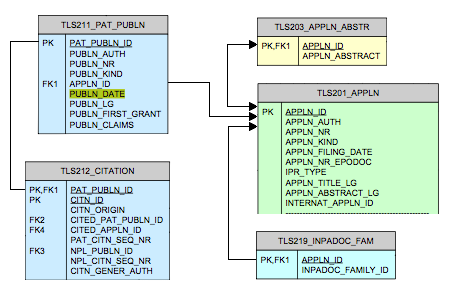
\includegraphics[width=130mm,scale=0.45]{Figures/psql_schema}
\decoRule
\caption[PSQLSchema]{Schema of PostgreSQL database containing relevant tables}
\label{fig:psqlSchema}
\end{figure}

% FORWARD CITATIONS
% how were forward citations calculated

% include  of subsetdatabase schema?
% stored in psql

\section{Data Pre-Processing}

%stopping, stemming, lower case, min_freq
The phrase "garbage in garbage out" is commonly used in machine learning to emphasize the importance of the data pre-processing step. We begin our pre-processing by retrieving abstracts from the aforementioned PSQL database and applying case folding such that words like "Turbine" at the beginning of a sentence will match the word "turbine" elsewhere. We then remove unnecessary symbols and punctuation via regex and apply stopping using the English \keyword{NLTK} stopwords list. This effectively removes common conjunctions and operational words from our corpus that don't actually contribute to the topics, such as "but, if, the, and" etc. 

[one line flow chart of pre-processing precedure?]

We then further distill the abstracts by applying lemmatization. This step is meant to reduce inflectional forms of a word such as "operates, operating, operational" to a base form "operate". After lemmatization, we remove any words occurring less than 25 times total, matching the implementation found in \parencite{Blei:2006:DTM:1143844.1143859}. Finally, we save the resulting corpus, totaling over 6,400 documents, and serialize the dictionary of vocabulary for subsequent access.

% number of unique words?

% used gensim, Python, Postgresql, ipython notebooks

\section{Tuning models}
Our selection of hyperparameters can have a large influence on the topics that models infer. For this reason, prior to running any of our experiments, we must take care in tuning the hyperparameters of our topic models, namely the number of topics $K$ and the maximum number of iterations $M_{iter}$.

\begin{table}
\caption{The effects of treatments X and Y on the four groups studied.}
\label{tab:treatments}
\centering
\begin{tabular}{l l l}
\toprule
\tabhead{Groups} & \tabhead{Treatment X} & \tabhead{Treatment Y} \\
\midrule
1 & 0.2 & 0.8\\
2 & 0.17 & 0.7\\
3 & 0.24 & 0.75\\
4 & 0.68 & 0.3\\
\bottomrule\\
\end{tabular}
\end{table}

To do this we defined a range of values for these parameters which we then sampled parameter sets from uniformly. At each parameter set we evaluated the umass, uci, npmi, and cv topic coherence of the resulting model. Table XXX contains the best parameter sets found for each model according to each coherence measure on a subset of documents. Figure \ref{fig:DTMcv} displays the cv coherences of the DTM as a function of $K$ and $M_{iter}$. From this plot we can see that increasing the number of topics $K$ beyond a certain point fails to improve topic coherence with similar results for the number of iterations.

\begin{figure}[h]
\centering
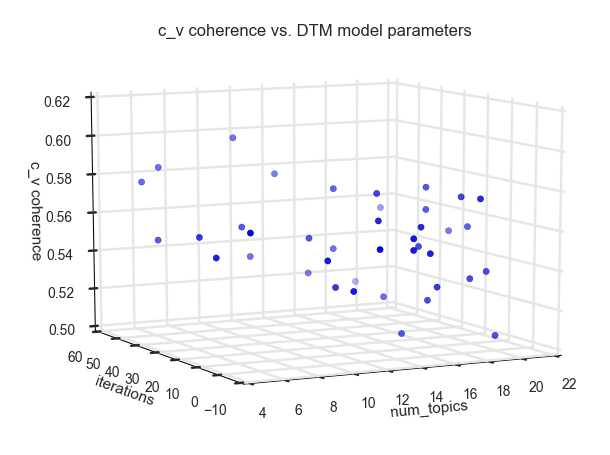
\includegraphics[width=130mm,scale=0.45]{Figures/DTMcvtuning}
\decoRule
\caption[DTMCV]{cv coherence values for DTM as a function of $K$ and $M_{iter}$}
\label{fig:DTMcv}
\end{figure}

you can see from the plot that (some comment or observation here.)

Ultimately went with cv recommended parameter sets as it correlated the highest with human judgement in (reference here)


% how we tested for coherence
setting the alpha parameter in LDA as recommended by (e.g., as in Steyvers and Griffiths 2007) It acts as a form of regularization.
A recommended setting is a = 50/K (Griffiths and Steyvers 2004; Steyvers and Griffiths 2007)

\section{Classification Set Up}
% how we classified 


\section{Clustering Set Up}
% how we carried out clustering



